Validating timing-models, especially those that may not have a strict
specification, is a fundamentally difficult proposition. Models like Ramulator
and DRAMsim2 can claim a strong degree of validation checking their generated
command stream with an RTL golden model that detects DRAM timing violations.
Since our DRAM models do not model refresh, we cannot re-use this strategy.
Lacking a "golden" specification against which to validate our models, we
employ three strategies to check our models:

\begin{enumerate}
    \item \textbf{Validation against a manually-written C++ model.} The C++ model forms a
        specification against which the instance is checked. Here, we drive both the
        C++ model and an RTL simulation of the instance with the same memory
        traces and compare the cycle-by-cycle behavior.

    \item \textbf{Sanity checking against DRAMSim2.} Here, we replace the C++
        model with a reference model (DRAMSim2). As before, we present
        identical memory traces to the reference and instance and compare
        the cycle-by-cycle behavior, and assess the degree to which they differ.

    \item \textbf{Sanity checking at the system-level.} In FPGA simulation, we run
        micro-benchmarks on the target whose memory-system behavior can be
        deduced \textit{a priori}.
\end{enumerate}

\begin{figure}[t]
	\centering
	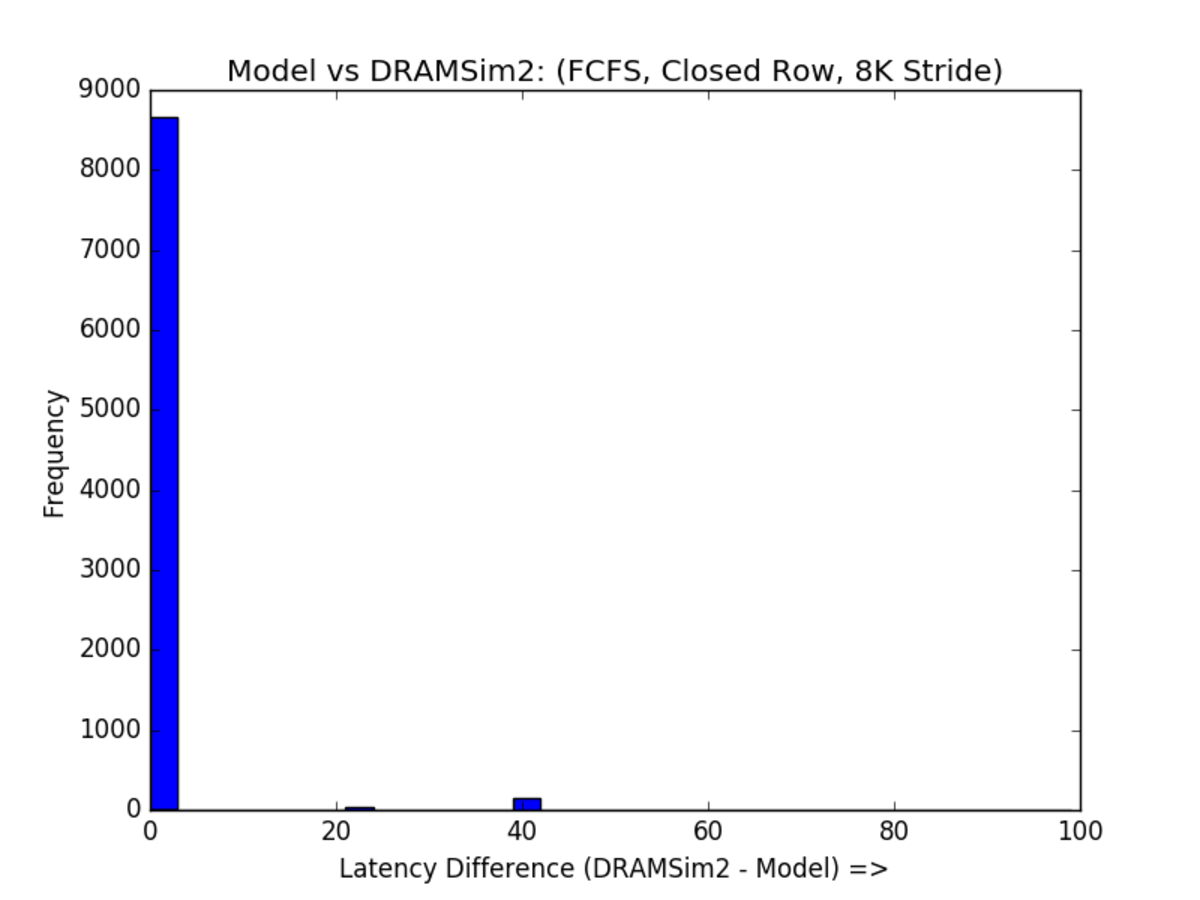
\includegraphics[width=0.75\columnwidth]{figures/close_row_stride.pdf}
    \caption{Histogram of latency-differences between our FCFS MAS model and DRAMSim2 (8 Banks, 8K pages, 9:1 read:write ratio,  $T_{RP},T_{CS},T_{RCD} =
    10$). Timing abberations are due to refresh.}
  \label{fig:error_histogram}
\end{figure}

While these techniques are sufficient to show that the models capture important
trends when sweeping a configuration setting, future work could explore a closer
comparison of our model against a cycle-accurate model like DRAMSim2.

Figure~\ref{fig:error_histogram}, illustrates the effect of refresh even when
the model is being driven lightly (periodic requests every 50 cycles) in trace
driven mode. We intend to employ more exhaustive validation against these
simulators as additional features are added to our models.

